\documentclass[a4paper,10pt]{article}
\usepackage[top=0cm,nohead,nofoot]{geometry}
\usepackage{fullpage}
\usepackage{graphicx}
\usepackage{amsmath}
\usepackage{url}
\usepackage{syntax}
\usepackage{listings}
\usepackage{hyperref}
\hypersetup{
    colorlinks,
    citecolor=black,
    filecolor=black,
    linkcolor=black,
    urlcolor=black
}

\begin{document}

\title{Inducing Probabilistic Programs by Bayesian Program Merging}
\author{Irvin Hwang\\Stanford University  \and Andreas Stuhlm\"{u}ller\\MIT \and Noah D. Goodman\\Stanford University}
\date{}
\maketitle
\vspace*{-2em}
\begin{abstract}

This report outlines an approach to learning generative models from data, when those models are represented as probabilistic programs. Expressing models as programs captures abstract patterns contained in the examples, such as stochastic recursion and parametrized sub-parts. Yet we don�t sacrifice concreteness: by choosing our language for programs to be an extension of the algebraic data type of the examples, we can begin with a program that generates all and only the examples, introducing greater abstraction, and generalization, incrementally to the extent that it is explanatory. 
Motivated by previous approaches to model merging and program induction, we search for such explanatory abstractions using program transformations.
%Formulating model learning in terms of program induction suggests that we can understand patterns as repeated computations within these programs. 
%This idea provides a unifying theme for searching the space of generative models, suggesting search moves that, in the spirit of Bayesian model merging, are based on program transformations. 
We consider two types of program transformation: The first is based on merging common subexpressions within a program into new function abstractions (anti-unification). The second simplifies functions by reducing the number of arguments. We demonstrate that this approach finds key patterns in the domain of nested lists, including: parametrized sub-functions and stochastic recursion.

\end{abstract}


\tableofcontents

\section{Introduction}

%% FIXME: more intro here

What do you see when you look at figure \ref{fig:plants}? What kinds of patterns are in the image? 
\begin{figure}[h]
\begin{center}
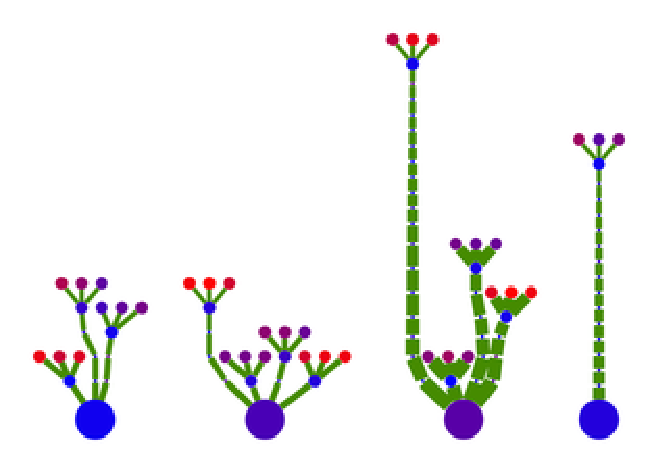
\includegraphics[scale=.60]{trees.pdf}
\end{center}
\caption{Tree-like objects.}
\label{fig:plants}
\end{figure}

You might describe the image as a series of trees where each tree has a large base and a number of branches of variable length with each branch ending in a flower that is either red or purple. Each part of this description corresponds to a different pattern detected in the image.  Recognizing patterns like these is an important aspect of intelligence; understanding algorithms that can identify such patterns will contribute to understanding human intelligence and extending the scope of machine intelligence.  
One way to approach this problem is as learning generative models for observed examples: we wish to find a description of the process that could have given rise to a set of examples, and will form this description in a rich language for generative processes---a probabilistic programming language. 
In this document, we build on the representation in \cite{A.Stuhlmueller:2010:6d11a} and explore a family of algorithms for learning probabilistic programs.

%A difficulty with the identification of regularities in data is that there are many notions of what it means to be a pattern and how this can vary with the types of data being analyzed.  We will approach this problem by first transforming data (whatever its type) into a canonical form (an expression in a programming language) and then defining pattern as repeated computation in this program.  


%some high-level discussion here, about what kinds of patterns are important to find, and needing a language that spans from very concrete to fully abstract?

The main components of our approach are as follows: representation of data in terms of algebraic data types, representation of patterns in data as probabilistic programs, guiding search through program space using the Bayesian posterior probability, and creating search moves by detecting repeated computation.  The general algorithm can be summarized as 
(1) turn the data into a large program that generates all and only the examples 
(2) identify (approximately) repeated structure in the large program and transform the program to make sharing explicit   %does this describe dearg well?
(3) continue, accepting transformations that increase the posterior probability of the program given the data.  
The probabilistic programs learned in such a manner can be understood as generative models and reasoning about such models can be formulated in terms of probabilistic inference. We illustrate these ideas on list-structured data.

Generative models play a prominent role in modern machine learning and understanding different classes of models, e.g., Hidden Markov models and probabilistic context-free grammars, have led to a wide variety of applications.  There is a trade-off between the variety of patterns a model class is able to capture and the feasibility of learning models in that class \cite{Russell2003}.  Much of machine learning has focused on studying classes of models with limited expressiveness in order to develop tractable algorithms for modeling large data sets.  Our investigation takes a different approach and explores how learning might proceed in a very expressive class of models with a focus on identifying abstract patterns from very small amounts of data.

In particular, we examine a class of generative models that are represented as programs in a probabilistic programming language. A probabilistic program represents a probability distribution, and each evaluation of the program results in a sample from the distribution. We implement these programs in a subset of the probabilistic programming language Church \cite{N.D.Goodman:2008:f2a0d}.  
These programs can have parameterized functions and recursion, which allow for natural representation of ``long-range'' dependencies and recursive patterns.  We will frame searching this space of models in terms of Bayesian model merging \cite{Stolcke:1994:IPG:645515.658235} and demonstrate that this approach can find interesting patterns in the list data domain.

Before we proceed, a note about what this report is and is not: This report \emph{is} a status update on our working system, containing detailed code and illustrative examples. It documents some progress we have made that we believe can be useful more generally.
This report \emph{is not} a completed academic work. In particular, it does little to situate our work within the context of previous work (some of which has  directly inspired us), provides little high-level discussion, and aims for illustrative examples rather than compelling applications.

\subsection{Bayesian model merging}

Bayesian model merging is a framework for searching through a space of generative models in order to find a model that accurately generates the observed data.  The main idea is to search model space through a series of merge transformations and to use the posterior $P(M|D)$ of model $M$ given data $D$ as a criterion for selecting transformations.

We create an initial model by building a program that has a uniform distribution over the training set ({\em data incorporation}).  While this initial model has high likelihood $P(D|M)$, it will never generate points outside the training set--it severely overfits the initial data.  Alternative model hypotheses are explored by transforming the initial model with merge operations.  Merge operations collapse the structure of a model (with specific details depending on the model class), and the resulting program often has better generalization properties.  

This technique has been successfully applied to learning artificial probabilistic grammars where the grammars were represented as hidden Markov models, n-grams, and probabilistic context-free grammars \cite{Stolcke:1994:IPG:645515.658235}. Our work differs in that we use a significantly richer model class of probabilistic programs.  This allows for more complex patterns to be represented as well as allowing for more types of transformations, including transformations that correspond to lossy compression of the data.


\subsection{Bayesian program merging}

%% FIXME: could improve decomposition

In order to use Bayesian program merging, we need to specify the following parts:

\begin{description}
\item[Data and language] Data is represented in terms of an algebraic data type, which gives us a way to form initial programs using the type constructors.  Programs are written in a formal language that consists of type constructors and additional operators.
\item[Probabilistic programs]  Distributions over data can be represented with probabilistic programs and the structure of the programs corresponds to regularities in the data.
\item[Search] Search is based on identifying programs with a high posterior probability and then applying transformations to these programs to continue exploration.
\item[Merge operations] Transformations on programs merge program structure, which can increase generalization of the model as well as its prior probability.
\end{description}


\newpage
\section{Data representation, algebraic data types, and language}
We assume that the data we deal with can be modeled with an algebraic data type whose constructors are known to us.  This assumption gives us a starting point for program induction, since any data can be directly translated into a program which is a derivation (sequence of constructor operations) of the data from the type specification. 
\subsection{Representation of data and programs in the domain of nested lists}
We can model the trees shown in figure \ref{fig:plants} in terms of nested lists (s-expressions).  Each tree consists of nodes, where each node has a size and color along with a list of child nodes.
\begin{grammar}
<tree> ::= nil

<tree> ::= (node <data> <tree> <tree> ... )

<data> ::= (data <color> <size>)

<color> ::= (color [number])

<size> ::= (size [number])
\end{grammar}
The following is an example of a tree expression along with a graphical representation.
\lstset{basicstyle=\small\ttfamily, frameround=fttt, breaklines=true, language=Lisp, showstringspaces=false, breakatwhitespace=true}
\begin{lstlisting}[mathescape=true]
(node (data (color 50) (size 1))
  (node (data (color 30) (size 0.3))
    (node (data (color 225) (size 0.3)))
    (node (data (color 225) (size 0.3)))
    (node (data (color 225) (size 0.3)))))
 $
\includegraphics[scale=1.0]{tree.pdf}$ 
\end{lstlisting}

We now have a way of representing data as rudimentary programs.  In order to capture interesting patterns, we need a more expressive language.  We use the following subset of Church for Bayesian program merging in the tree domain:
\begin{grammar}
<expr> ::= (begin <expr> <expr> ... ) 
\alt (lambda (<var> ...) <expr>)
\alt (<expr> <expr>)  
\alt (define <var> <expr>)
\alt (if (flip [number]) <expr> <expr>)
\alt <var> 
\alt <primitive>

<var> ::= V[number] | F[number] 

<primitve> ::= uniform-choice | list | node | data | color | size | [number]
\end{grammar}

\subsection{Data incorporation}
The first step of Bayesian program merging is data incorporation.  Data incorporation is the creation of an initial model by going through each example in the training set and creating an expression that evaluates to this example (in terms of the algebraic data type constructors).  These programs are combined into a single expression that draws uniformly from this list. 
% We assume Gaussian noise in the color attribute for simplicity's sake, but discuss a possible direction for learning such a property later in the report.
\begin{lstlisting}[frame=trBLsingle]
(define (incorporate-data trees)
  `(lambda () (uniform-choice ,@(map tree->expression trees))))

(define (tree->expression tree)
  (if (null? tree)
      '()
      (pair 'node (pair (node-data->expression (first tree)) 
                        (map tree->expression (rest tree))))))

(define (node-data->expression lst)
  `(data (color (gaussian ,(first (second lst)) 25)) 
	 (size ,(first (third lst)))))
\end{lstlisting}
In the implementation the data are unannotated s-expressions (an example being \texttt{(((1) (2)))}), which can be trivially converted into an expression in terms of the tree type constructors (the tree expression for the above example is \texttt{(node (data (color 1) (size 2)))}).  In this report, we assume for readability that all data is given in tree expression form. An important question we leave for future work is how to perform data incorporation when the data is less structured, e.g., feature vectors.  If we give \texttt{incorporate-data} the input: 
\begin{lstlisting}[mathescape=true]
((node (data (color 70) (size 1))
       (node (data (color 37) (size 0.3))
             (node (data (color 213) (size 0.3)))
             (node (data (color 207) (size 0.3)))
             (node (data (color 211) (size 0.3)))))
 (node (data (color 43) (size 1))
       (node (data (color 47 25)) (size 0.1))
             (node (data (color 33) (size 0.3))
                   (node (data (color 220) (size 0.3)))
                   (node (data (color 224) (size 0.3)))
                   (node (data (color 207) (size 0.3)))))))
$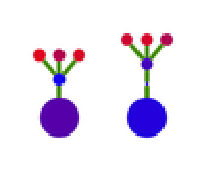
\includegraphics[scale=.7]{initData.pdf}$
\end{lstlisting}

We get the program 
\begin{lstlisting}[mathescape=true]
(lambda ()
  (uniform-choice
   (node (data (color (gaussian 70 25)) (size 1))
         (node (data (color (gaussian 37 25)) (size 0.3))
               (node (data (color (gaussian 213 25)) (size 0.3)))
               (node (data (color (gaussian 207 25)) (size 0.3)))
               (node (data (color (gaussian 211 25)) (size 0.3)))))
   (node (data (color (gaussian  43)) (size 1))
         (node (data (color (gaussian 47 25)) (size 0.1))
               (node (data (color (gaussian 33 25)) (size 0.3))
                     (node (data (color (gaussian 220 25)) (size 0.3)))
                     (node (data (color (gaussian 224 25)) (size 0.3)))
                     (node (data (color (gaussian 207 25)) (size 0.3))))))))
$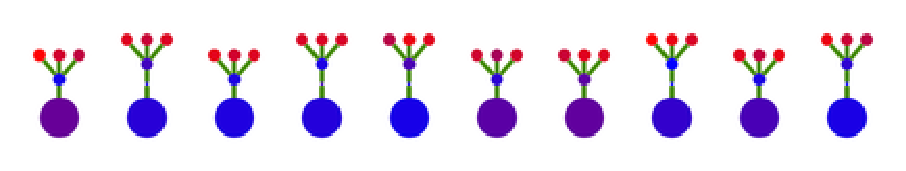
\includegraphics[scale=.7]{initProgram.pdf}$
\end{lstlisting}


\newpage
\section{Probabilistic programs}
A generative model is a joint probability distribution over latent states and observed data. We can represent such a joint distribution as a program in a probabilistic programming language like Church \cite{N.D.Goodman:2008:f2a0d}. The structure of the program, i.e., the decomposition into functions and the flow of control, can capture regularities in the data. We illustrate this idea by looking at a probabilistic program that generates the images in figure \ref{fig:plants}. Different parts of the program correspond to the different patterns we described earlier (functions and variables are given semantically meaningful names for readability, but can easily be replaced by F[number] and V[number] to fit the grammar specified earlier).  
\begin{lstlisting}[mathescape=true]
(define (tree)
  (uniform-choice
   (node (body) (branch))
   (node (body) (branch) (branch))
   (node (body) (branch) (branch) (branch))
   (node (body) (branch) (branch) (branch) (branch))))

(define (body) 
  (data (color (gaussian 50 25)) (size 1)))

(define (branch)
  (if (flip .2) 
      (flower (if (flip .5) 150 255))
      (node (branch-info) (branch))))

(define (branch-info)
  (data (color (gaussian 0 25)) (size .1)))

(define (flower shade)
  (node (data (color (gaussian 0 25)) (size .3))
        (petal shade)
        (petal shade)
        (petal shade)))

(define (petal shade)
  (node (data (color shade) (size .3))))
$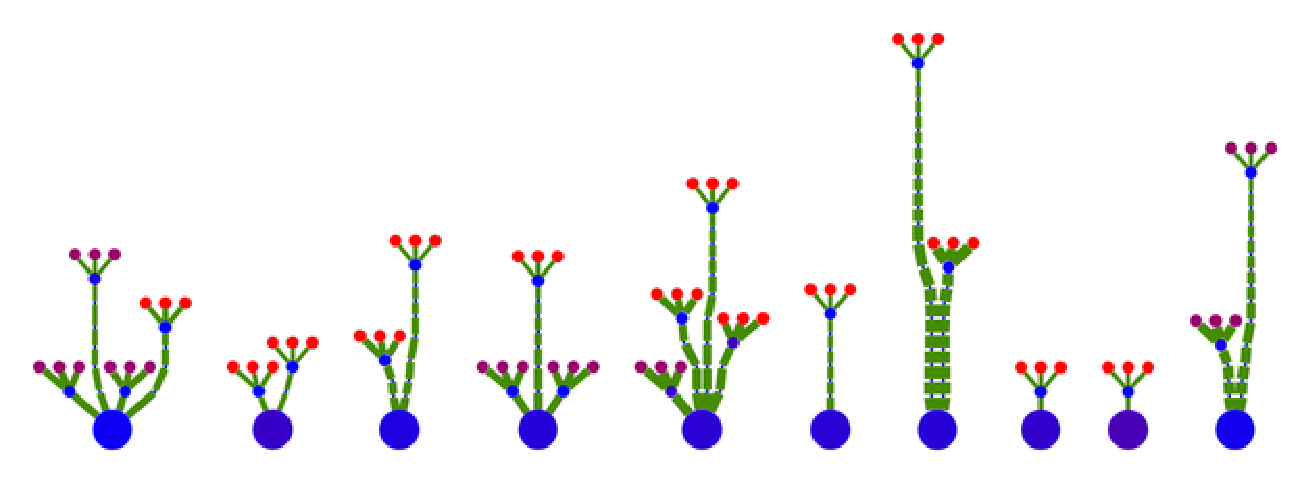
\includegraphics[scale=.35]{trees2.pdf}$
\end{lstlisting}
We can think programs as a combination of data constructor operations with some additional control flow operations and lambda abstractions.  The above tree program begins by determining the number of branches the tree will have and then creates a large body node that connects these branches.  Each branch function recursively connects a series of small nodes together and ends in a call to the flower function, passing it one of two colors.  The flower function creates a node with three ``petal'' nodes each of the same color.  Looking at this program we see how patterns such as a flower having three petals and the body having a large base are reflected in the program structure.  The compositionality of the language also captures relational patterns such as branches end in flowers.  Now that we know many different patterns can be represented within a probabilistic program, the main question becomes how do we change the structure of our initial data incorporated program to reflect such patterns.

\subsection{Data abstractions}
We use data abstractions for programs and functions created by merge operations on programs.  A function created by a merge operation is called an abstraction (after lambda abstraction).  It consists of a name, variables, and a pattern, i.e., the s-expression that makes up the body of the function.  
\begin{lstlisting}[frame=trBL]
(define (make-abstraction body variables)
  (make-named-abstraction (sym FUNC-SYMBOL) body variables))
(define (make-named-abstraction name body variables)
  (list 'abstraction name variables body))

(define abstraction->name second)
(define abstraction->vars third)
(define abstraction->body fourth)
\end{lstlisting}
Here \texttt{sym} is used to create unique symbols in an orderly manner for use as function or variable names.


Programs represent the generative models we search over.  They consist of a list of abstractions and a body.
\begin{lstlisting}[frame=trBL]
(define (make-program abstractions body)
  (list 'program abstractions body))
(define program->abstractions second)
(define program->body third)
\end{lstlisting}  

We use a wrapper around the programs to keep track of additional program information during search.  The motivation for this additional information will become clearer after reading the next section on beam search, but the basic idea is if a program's semantics are preserved after a transformation, the likelihood does not need to be recomputed (an expensive computation). The additional information in the wrapper is bookkeeping used to exploit this fact during search.  
\begin{lstlisting}[frame=trBL]
(define (make-program+ program posterior log-likelihood log-prior semantics-preserved)
  (list 'program+ program posterior log-likelihood log-prior 
        semantics-preserved))
(define program+->program second)
(define program+->posterior third)
(define program+->log-likelihood fourth)
(define program+->log-prior fifth)
(define program+->semantics-preserved sixth)
(define (program+->program-transform semantics-preserved program+ new-program)
  (make-program+ new-program 
                 (program+->posterior program+) 
                 (program+->log-likelihood program+) 
                 (program+->log-prior program+) 
                 semantics-preserved))
\end{lstlisting}


\subsection{Posterior probability}
An important aspect of using probabilistic programs is they represent computable probability distributions or generative models.  This means we can talk about the posterior probability distribution of a program, which is defined by Bayes theorem as 
\begin{equation}P(M|D)\propto P(D|M)P(M)\end{equation}
Where $P(D|M)$ is the probability of data $D$ being generated by program $M$, also known as the likelihood, and $P(M)$ is the probability of a program, also known as the prior.

We use a prior based on program length like in Bayesian model merging.  
\begin{equation}P(M)\propto e^{-\alpha size(M)}\end{equation}
\begin{lstlisting}[frame=trBL]
(define (log-prior program)
  (- (alpha * (program-size program))))
\end{lstlisting}
This prior effectively biases the search towards smaller programs.  Increasing the constant $\alpha$ gives the prior more weight when calculating the posterior, which means minimizing program size becomes more important.  A program's size is the number of symbols in the function bodies as well as the main body.
\begin{lstlisting}[frame=trBL]
(define (program-size program)
  (define (sexpr-size sexpr)
    (if (list? sexpr)
        (apply + (map sexpr-size sexpr))
        1))
  (define (abstraction-size abstraction)
    (sexpr-size (abstraction->body abstraction)))
  (let* ([abstraction-sizes (apply + (map abstraction-size (program->abstractions program)))]
         [body-size (sexpr-size (program->body program))])
    (+ abstraction-sizes body-size)))
\end{lstlisting}
The computation of the likelihood is the difficult part in estimating the posterior.  Intuitively we can think of it as way to say how good a particular program is at producing a set of target data.  This is important in search because it can give information on whether and/or how to adjust our hypothesis.  In a deterministic setting where the programs do not have randomness we can often have an intuitive sense of whether a program is good or bad based on some metric we make up on the space of outputs and the data.  Working in the probabilistic setting allows us to have a more standard way of deciding whether a program is good or bad.  The main idea being a probabilistic program is a generative process and represents a distribution over possible data.  Given the ``right'' random choices during the execution of the program the output will be the observed data.  By knowing the probabilities of these choices, we can combine them based on the rules of probability to get a score for how likely our program is to generate the observed data and this gives us a sense of whether the program is good or bad.  There may be many possible settings for the random choices of a program and this can make determining which choices lead to the observed data difficult.  There is an additional difficulty in that there could be many possible settings that lead to the observed data and we need to take take all of them into account.  We give an example of one possible way to approximate this computation for list-type data in the example below.
\subsection{Likelihood estimation in the list domain}
In the case of programs that generate list-structured data we can estimate the likelihood by splitting the data into the discrete topology of the list and its continuous items.  We begin by factoring the problem in the following way:
\begin{eqnarray}
P(ts|p) &=& \prod_{ts}P(t|p)
\end{eqnarray}
where $ts$ stands for trees, our target data, the $t$ stands for a single tree, and $p$ is the program.
\begin{lstlisting}[frame=trBL]
(define (log-likelihood trees prog sample-size)
  (apply + (map (lambda (tree) (single-log-likelihood prog sample-size tree)) trees)))
\end{lstlisting}
The idea behind estimating the likelihood for a single tree, $P(t|p)$, is to evaluate the program several times forcing the computation to result in the target tree each time.  Each evaluation gives a probability for a possible way of generating the tree from the model.  This probability is the product of random choices made in the program during evaluation.  Since there may be several possible ways to generate the tree from the program we average the different evaluations.  In the code below \texttt{smc-core} (where smc stands for sequential Monte Carlo) is the part that forces evaluation of the program to the desired data.  A detailed description of \texttt{smc-core} is beyond the scope of this report, but it can be thought of as an incremental forward sampling process.  Due to the forward-sampling nature of this process, we separate random choices used in generating the continuous-valued parts of the tree (i.e., the color) from the random choices that influence the tree structure.
\begin{lstlisting}[frame=trBL]
(define single-log-likelihood 
   (lambda (program popsize tree)
     (let* ([new-program (replace-gaussian (desugar program))]
            [model (eval (program->sexpr new-program))]
            [topology-scores+tree-parameters (compute-topology-scores+evaluate model tree popsize)]
            [topology-scores (first topology-scores+tree-parameters)]
            [trees-with-parameters (second topology-scores+tree-parameters)]
            [data-scores (map (lambda (tree-with-parameters) (compute-data-score tree tree-with-parameters)) trees-with-parameters)] ;;remove -inf?
            [scores (delete -inf.0 (map + topology-scores data-scores))]
            [score (if (null? scores)
                        -inf.0
                        (apply log-sum-exp scores))])
       score)))
\end{lstlisting}
We take advantage of the fact we can directly compute the probability of a sample from a Gaussian given the parameters.  We do this by modifying the Gaussian functions in the program to output the mean and variance for a particular node rather than sampling a value from the distribution.  The code below also changes the uniform-choice syntactic construct into a uniform-draw, which is part of standard Church.
\begin{lstlisting}[frame=trBL]
(define (replace-gaussian program)
  (define (gaussian? sexpr)
    (tagged-list? sexpr 'gaussian))
  (define (return-parameters sexpr)
    `(list 'gaussian-parameters ,(second sexpr) ,(third sexpr)))
  (define (replace-in-abstraction abstraction)
    (make-named-abstraction (abstraction->name abstraction) (sexp-search gaussian? return-parameters (abstraction->pattern abstraction)) (abstraction->vars abstraction)))
  (let* ([converted-abstractions (map replace-in-abstraction (program->abstractions program))]
	 [converted-body (sexp-search gaussian? return-parameters (program->body program))])
    (make-program converted-abstractions converted-body)))

(define (desugar program)
  (define (uniform-choice? sexpr)
    (tagged-list? sexpr 'uniform-choice))
  (define (uniform-draw-conversion sexpr)
    `((uniform-draw (list ,@(map thunkify (rest sexpr))))))
  (define tests+replacements (zip (list uniform-choice?) (list uniform-draw-conversion)))
  (define (apply-transforms sexpr)
    (fold (lambda (test+replacement expr)
	    (sexp-search (first test+replacement) (second test+replacement) expr))
	  sexpr
	  tests+replacements))
  (define (desugar-abstraction abstraction)
    (make-named-abstraction (abstraction->name abstraction) (apply-transforms (abstraction->pattern abstraction)) (abstraction->vars abstraction)))
  (let* ([converted-abstractions (map  desugar-abstraction (program->abstractions program))]
	 [converted-body (apply-transforms (program->body program))])
    (make-program converted-abstractions converted-body)))

(define (thunkify sexpr) `(lambda () ,sexpr))
\end{lstlisting}
The modified program is evaluated several times to generate trees whose topology (node structure) matches the observed tree and has the parameters for the Gaussian used to generate a color.  During the evaluation of the modified program we also capture the probability for the choices made in generating the topology of the tree.  
\begin{lstlisting}[frame=trBL]
(define (compute-topology-scores+evaluate model tree popsize)
  (let* ([smc-core-arguments (create-smc-core-args model tree popsize)]
         [samples (apply smc-core smc-core-arguments)]
         [repeat-symbol (find-repeat-symbol samples)]
         [samples
          (fold (lambda (s a)
                  (if (member (mcmc-state->addrval s repeat-symbol)
                              (map (lambda (x) (mcmc-state->addrval x repeat-symbol)) a))
                      a (pair s a))) '() samples)]
         [topology-scores (map mcmc-state->score samples)]
         [generated-trees (map mcmc-state->query-value samples)])
    (list topology-scores generated-trees)))
\end{lstlisting}
We can use the Gaussian parameters for each node's color to determine the probability of the observed color values of a tree.
\begin{lstlisting}[frame=trBL]
(define (compute-data-score tree tree-with-parameters)
    (if (null? tree)
        0
        (+ (single-data-score (node->data tree) (node->data tree-with-parameters)) (apply + (map compute-data-score (node->children tree) (node->children tree-with-parameters))))))

(define (single-data-score original-data parameterized-data)
  (let* ([color-score (score-attribute (data->color original-data) (data->color parameterized-data))]
         [size-score (score-attribute (data->size original-data) (data->size parameterized-data))])
    (+ color-score size-score)))

(define (score-attribute original-attribute parameterized-attribute)
  (if (tagged-list? parameterized-attribute 'gaussian-parameters)
      (log (normal-pdf (first original-attribute) (gaussian->mean parameterized-attribute) (gaussian->variance parameterized-attribute)))
      (if (= (first original-attribute) (first parameterized-attribute)) 0 -inf.0)))

(define gaussian->mean second)
(define gaussian->variance third)
\end{lstlisting}


\newpage
\section{Bayesian search}

We are interested in programs with high posterior probability. Many different search strategies are possible, but in this report, we limit ourselves to beam search using the posterior probability as a search heuristic.

\begin{lstlisting}[frame=trBL]
(define (beam-search data init-program beam-size depth)
  (let* ([top-transformations 
          (sort-by-posterior
           data 
           (beam-learn-search-transformations data init-program beam-size depth))])
    (if (null? top-transformations)
        init-program
        (program+->program (first top-transformations)))))

(define (beam-search-transformations data program beam-size depth)
  (let ([init-program+ (make-program+ program 0 (log-likelihood data program 10) (log-prior program) #f)])
    (depth-iterated-transformations (lambda (programs+) (best-n data programs+ beam-size)) init-program+ depth)))

(define (best-n data programs+ n)
  (max-take (sort-by-posterior data programs+) n))
\end{lstlisting}
The main part of the search is performed by \texttt{depth-iterated-transformations}, which recursively applies program transformations to the best programs at a given search depth and then filters the results to get the best programs for the next depth.
\begin{lstlisting}[frame=trBL]
(define (depth-iterated-transformations cfilter program+ depth)
  (let* ([transformed-programs+ (apply-and-filter-transformations depth cfilter program+)])
    (delete '()  (append transformed-programs+
                         (apply append (map (lambda (prog) 
                                              (depth-iterated-transformations cfilter prog (- depth 1))) 
                                            transformed-programs+))))))
\end{lstlisting}
We reduce the amount of computation required when choosing the best programs at each level of search by separating program transformations that preserve semantics from those that do not.  Marking programs based on their transformation type allows us to reuse likelihood for a program that was created by a semantics preserving transformation.
\begin{lstlisting}[frame=trBL]
(define (apply-and-filter-transformations depth cfilter program+)
  (if (= depth 0)
      '()
      (let* ([semantics-preserved-programs+ (apply-transformations program+ semantic-preserving-transformations #t)]
             [semantics-changed-programs+ (apply-transformations program+ semantic-changing-transformations #f)])
        (cfilter (append semantics-preserved-programs+ semantics-changed-programs+)))))

(define (apply-transformations program+ transformations semantics-preserving)
  (let* ([program (program+->program program+)]
         [transformed-programs (delete '() (concatenate (map (lambda (transform) (transform program #t)) transformations)))]
         [transformed-programs+ (map (lambda (program) (program+->program-transform semantics-preserving program+ program)) transformed-programs)])
    transformed-programs+))
\end{lstlisting}
The posterior distribution is estimated by combining an estimate of the likelihood with the computation of the prior.  
\begin{lstlisting}[frame=trBL]
(define (sort-by-posterior data programs+)
  (let* ([programs (map program+->program programs+)]
         [semantics-flags (map program+->semantics-preserved programs+)]
         [log-priors (map log-prior programs)]
         [log-likelihoods (map (lambda (prog+ semantics-flag)
                                 (if semantics-flag
                                     (program+->log-likelihood prog+)
                                     (log-likelihood data (program+->program prog+) 10))) programs+ semantics-flags)]
         [posteriors (map + log-priors log-likelihoods)] 
         [new-programs+ (map make-program+ programs posteriors log-likelihoods log-priors semantics-flags)]
         [posteriors> (lambda (a b) (> (program+->posterior a) (program+->posterior b)))])
    (my-list-sort posteriors> new-programs+)))
\end{lstlisting}


\newpage
\section{Merge operations}
We described earlier how patterns in the program representation of data can be viewed as repeated computation.  Here we describe how this idea manifests itself as concrete program transformations used in exploring the search space.

\subsection{Inverse inlining}
Inlining is the process of replacing function calls in a program with the body of the function called.  inverse inlining creates new functions based on syntactic patterns in a program and replaces these patterns with calls to the newly created functions.  We can think of this process as creating lambda abstractions that potentially compress the program by removing duplication in the code and acts as a proxy for recognizing repeated computation.  The following code fragment outlines this procedure where compressions finds the different (lambda) abstractions that can be formed by anti-unifying (partially matching) pairs of subexpressions in a condensed form of the program (only the bodies of the functions and the body of the program).  Duplicate abstractions are filtered out then transformed programs are created by inverse inlining function calls for each of the abstractions.  

\begin{lstlisting}[frame=trBL]
(define (compressions program . nofilter)
  (let* ([condensed-program (condense-program program)]
         [abstractions (possible-abstractions condensed-program)]
         [compressed-programs (map (curry compress-program program) abstractions)]
         [prog-size (program-size program)]
         [valid-compressed-programs
          (if (not (null? nofilter))
              compressed-programs
              (filter (lambda (cp) (<= (program-size cp)
                                  (+ prog-size 1)))
                      compressed-programs))])
    valid-compressed-programs))

(define (condense-program program)
  `(,@(map abstraction->body (program->abstractions program))
    ,(program->body program)))

(define (possible-abstractions expr)
  (let* ([subexpr-pairs (list-unique-commutative-pairs (all-subexprs expr))]
         [abstractions (map-apply (curry anti-unify-abstraction expr) subexpr-pairs)])
    (filter-abstractions  abstractions)))
\end{lstlisting}

Aside from the obvious correspondence between repetition in program syntax and repetition in computation, there are two other reasons to believe that this is a useful transformation. In terms of Bayesian model merging we are merging the structure of the model, which potentially leads to models with better generalization properties \cite{Stolcke:1994:IPG:645515.658235}.  Inverse inlining can also also be interpreted as finding partial symmetries like in the work of Bokeloh et al. \cite{DBLP:journals/tog/BokelohWS10}, which was successful in the domain of inverse-procedural modeling.

The following example illustrates the inverse inlining transformation on a language slightly different from the tree example.
\begin{lstlisting}[mathescape=true]
(uniform-choice 
 (node
  (node a (node a (node b) (node b)))
  (node a (node a (node c) (node c)))))
$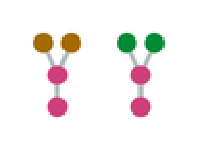
\includegraphics[scale=.40]{csrExample.pdf}$
\end{lstlisting}
a possible result of this transformation would be
\begin{lstlisting}[mathescape=true]
(begin
  (define (F1 V1 V2)
    (node a (node a (node V1) (node V2))))
  (uniform-choice (node (F1 b b) (F1 c c))))
$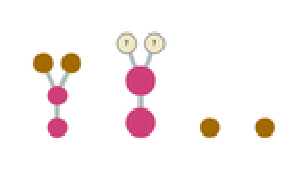
\includegraphics[scale=.40]{csrDecompose1.pdf}\\
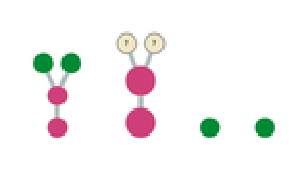
\includegraphics[scale=.40]{csrDecompose2.pdf}$
\end{lstlisting}
The first thing to note is both programs have the same behavior, i.e., this transformation is semantics preserving.  Both programs return either \texttt{(a (a (b) (b)))} or \texttt{(a (a (c) (c)))} with equal probability.

  The transformation can be described as refactoring subexpressions that partially match in a program with a function whose body is the common parts of the matching subexpressions.  In the above example the subexpressions that partially match are \texttt{(node a (node a (node b) (node b)))} and \texttt{(node a (node a (node c) (node c)))}.  The common subexpression is \texttt{(node a (node a (node x) (node y)))}, the function created using this common subexpression is \texttt{F1} and the original subexpressions are refactored as \texttt{(F1 b b)} and \texttt{(F1 c c)}.

An inverse inlining transformation can be created for each pair of subexpressions that have a partial match.  In the case of \texttt{(+ (+ 2 2) (- 2 5))} the following pairs of subexpressions have a partial match: \texttt{[2,2], [(+ 2 2), (- 2 5)], [(+ 2 2), (+ (+ 2 2) (- 2 5))]}.
\subsubsection{Anti-unification}
The process of finding a partial match between two expressions is called anti-unification.  One way to understand the process is in terms of the syntax trees for the expressions.  Every s-expression can be thought of as a tree where the lists and sublists of the s-expression make up the interior nodes and the primitive elements of the lists (e.g., symbols, numbers) are the leaves.  The tree in figure \ref{expressionTree} corresponds to the expression \texttt{(+ (+ 2 2) (- 2 5))}.  Finding a partial match between two expressions can be thought of as finding a common subtree between their tree representations.
\begin{figure}[h]
\begin{center}
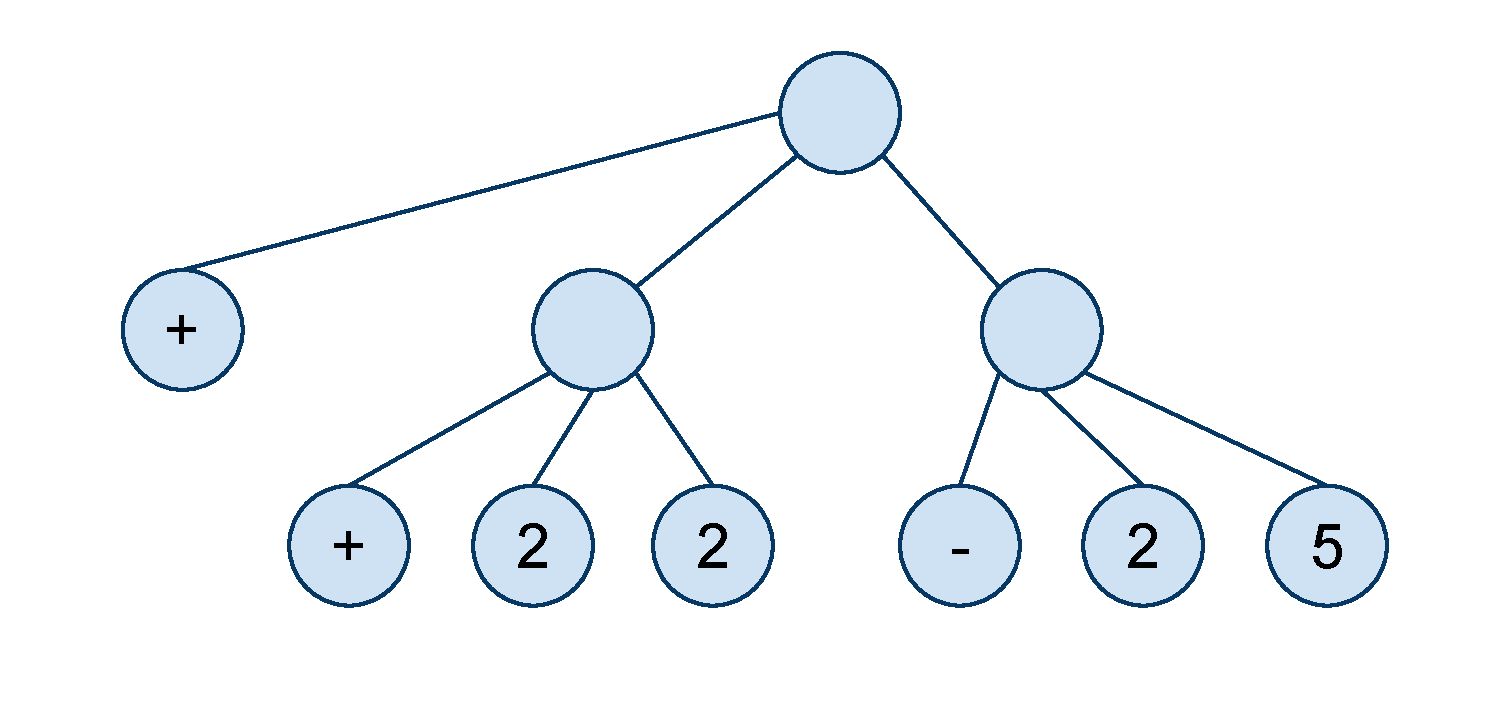
\includegraphics[scale=.40]{expressionTree.pdf}
\caption{An expression represented as a tree.}
\label{expressionTree}
\end{center}
\end{figure}

Anti-unification proceeds by recursively comparing two expressions, A and B (performed by \texttt{build-pattern}).  If A and B are the same primitive that primitive is returned.  If A and B are lists $(a_1,\ldots,a_n)$ and $(b_1,\ldots,b_n)$ of the same length then a list C $(c_1,\ldots,c_n)$ where each element $c_i$ is the anti-unification $a_i$ and $b_i$ is returned.  For all other cases when A and B do not match a variable is returned.

\begin{lstlisting}[frame=trBL]
(define anti-unify
  (lambda (expr1 expr2)
    (begin
      (define variables '())

      (define (add-variable!)
        (set! variables (pair (sym (var-symbol)) variables))
        (first variables))
      
      (define (build-pattern expr1 expr2)
        (cond [(and (primitive? expr1) (primitive? expr2)) (if (equal? expr1 expr2) expr1 (add-variable!))]
              [(or (primitive? expr1) (primitive? expr2)) (add-variable!)]
              [(not (eqv? (length expr1) (length expr2))) (add-variable!)]
              [else
               (let ([unified-expr (map (lambda (subexpr1 subexpr2) (build-pattern subexpr1 subexpr2))
                                        expr1 expr2)])
                 unified-expr)]))
      (let ([pattern (build-pattern expr1 expr2)])
        (list pattern (reverse variables))))))
\end{lstlisting}

{\bf Example} We illustrate the process of anti-unification on the expressions \texttt{(+ (+ 2 2) (- 2 5))} and \texttt{(+ (- 2 3) 4)}
The first step is to compare the root of the trees and make sure we have lists of the same size, in this case they are both of size three so we have a matching roots and a partial match of \texttt{(* * *)} where the *'s are yet to be determined.
Now we recursively attempt to match the three subexpressions + with +, \texttt{(+ 2 2)} with \texttt{(- 2 3)}, and \texttt{(- 2 5)} with 4.
Since + and + are both primitives that are the same they match, and our partial match is now \texttt{(+ * *)}.
Comparing \texttt{(+ 2 2)} and \texttt{(- 2 3)} we see that they are both lists of size 3 and so they match giving us a total partial match of \texttt{(+ (* * *) *)}.
Again we recursively match subexpressions of \texttt{(+ 2 2)} and \texttt{(- 2 3)}, i.e., + to -, 2 to 2, and 2 to 3.
Since + and - are primitives that do not match we replace them with a variable to get a total partial match of \texttt{(+ (V1 * *) *)}
Likewise after comparing 2 to 2 and 2 to 3 we get \texttt{(+ (V1 2 V2) *)} as our partial match.
In the final comparison of \texttt{(- 2 5)} and 4 we check can see there is no match because one \texttt{(- 2 5)} is a list and 4 is a primitive so the final result of our anti-unification is \texttt{(+ (V1 2 V2) V3)}.


\subsubsection{Refactoring programs}
Now that we have created lambda abstractions from the partial matches between two subexpressions of some program, P, we can use these abstractions to refactor P, possibly compressing it.  The idea will be to take the pattern of the abstraction (the body of the lambda abstraction) and replace any subexpressions of P that fit the pattern.  A subexpression that fits the pattern is replaced by an application of the lambda abstraction.  We first do this replacement for each of the functions in P and then the body, resulting in a program P'.  After all the replacements are made, the lambda abstraction is inserted into the set of functions for P' and this is our refactored program.
\begin{lstlisting}[frame=trBL]
(define (compress-program program abstraction)
  (let* ([compressed-abstractions (map (curry compress-abstraction abstraction) (program->abstractions program))]
         [compressed-body (replace-matches (program->body program) abstraction)])
    (make-program (pair abstraction compressed-abstractions)
                  compressed-body)))

(define (compress-abstraction compressor compressee)
  (make-named-abstraction (abstraction->name compressee)
                          (replace-matches (abstraction->body compressee) compressor)
                          (abstraction->vars compressee)))                           
\end{lstlisting}
Finding and replacing pattern matches of an abstraction F in an expression E proceeds recursively by taking the body of F and trying to match it to the expression on E.  A match between the body of the abstraction and the expression is determined by unification. If a match exists, then the application of F is returned where the arguments to F are refactored (if F has arguments).  If the match does not hold then E is returned with each of its subexpressions refactored.  If E is a primitive and not a match it is returned.

\begin{lstlisting}[frame=trBL]
(define (replace-matches s abstraction)
  (let ([unified-vars (unify s
                             (abstraction->body abstraction)
                             (abstraction->vars abstraction))])
    (if (false? unified-vars)
        (if (list? s)
            (map (lambda (si) (replace-matches si abstraction)) s)
            s)
        (pair (abstraction->name abstraction)
              (map (lambda (var) (replace-matches (rest (assq var unified-vars)) abstraction))
                   (abstraction->vars abstraction))))))
\end{lstlisting}

{\bf Example} In the case of \texttt{(+ (+ 2 2) (- 2 5))} the partial match resulting from anti-unification between the subexpressions \texttt{[(+ (+ 2 2) (- 2 5)), (+ 2 2)]} is \texttt{(+ V1 V2)}.  We refactor the original expression \texttt{(+ (+ 2 2) (- 2 5))} in terms of \texttt{(+ V1 V2)} by creating a function \texttt{(define (F1 V1 V2) (+ V1 V2))} and applying it in the expression.  For example one application could be \texttt{(F1 (+ 2 2) (- 2 5))} and another could be \texttt{(+ (F1 2 2) (- 2 5))}.  In general, we apply the function everywhere possible and get a refactored program such as:
\begin{lstlisting}
(+ (+ 2 2) (- 2 5))
=>
(begin
  (define (F1 V1 V2) (+ V1 V2))
  (F1 (F1 2 2) (- 2 5)))
\end{lstlisting}
The input to the refactoring procedure is a function, F, created from anti-unification and an expression, E, which will be refactored in terms of F.  In the example above F was \texttt{(define (F1 V1 V2) (+ V1 V2))}, E would be \texttt{(+ (+ 2 2) (- 2 5))}, and the result of refactoring was 
\begin{lstlisting}
(begin
  (define (F1 V1 V2) (+ V1 V2))
  (F1 (F1 2 2) (- 2 5)))
\end{lstlisting}

In the example \texttt{(+ (+ 2 2) (- 2 5))} matches \texttt{(+ V1 V2)} so an application of F1 to refactored arguments \texttt{(+ 2 2)} and \texttt{(- 2 5)} is returned resulting in \texttt{(F1 (F1 2 2) (- 2 5))}\footnote{Observe the function \texttt{F1} is basically the addition function between two numbers and so refactoring the program in terms of this function does compress the original expression at all.  An example where refactoring can compress an expression would be if the abstraction between \texttt{[(+ (+ 2 2) (- 2 5)), (+ 2 2)]} had been \texttt{(define (F1 V1) (+ V1 V1))}, then the refactored expression would be \texttt{(+ (F1 2) (- 2 5))}, which is one character smaller than \texttt{(+ (+ 2 2) (- 2 5))}.}.  


\subsubsection{Unification}
Determining whether there is a match between a function body and an expression is known as unification \cite{Robinson:1965:MLB:321250.321253}.  Earlier we described anti-unification which can be thought of as a process to create a pattern from two expressions, unification can be viewed as the opposite process of seeing if and how a given pattern fits onto an expression.  The return value of unification is a list of assignments for the variables of the function that would make the function the same as the expression.

The input to unification is a function F, and an expression E.  Unification occurs recursively by checking whether the body of F and E are lists of the same size.  If they are the same size then unification returns the unification of each of the subexpressions.  If they are not the same size or only one of them is a list unification returns false.  In the case where both expressions being unified are primitives true is returned if they are equal and false otherwise.  In the case where the function expression of the unification is a variable an assignment is returned, i.e., the variable along with the other expression passed to unification.  At the end a check is made to see if any unifications have returned false, in which case unification of F and E returns false.  There is also a check that any variable that is repeated in F has the same value assigned to it for each place it appears.  If this is not the case unification returns false. If unification is not false then an assignment for each unique variable of F is returned.

\begin{lstlisting}[frame=trBL]
(define unify
  (lambda (s sv vars)
    (begin
      (define (variable? obj)
        (member obj vars))

      ;;deals with a variable that occurs multiple times in sv
      (define (check/remove-repeated unified-vars)
        (let* ([repeated-vars (filter more-than-one (map (curry all-assoc unified-vars) (map first unified-vars)))])
          (if (and (all (map all-equal? repeated-vars)) (not (any false? unified-vars)))
              (delete-duplicates unified-vars)
              #f)))
      
      (cond [(variable? sv) (if (eq? s 'lambda) #f (list (pair sv s)))]
            [(and (primitive? s) (primitive? sv)) (if (eqv? s sv) '() #f)]
            [(or (primitive? s) (primitive? sv)) #f]
            [(not (eqv? (length s) (length sv))) #f]
            [else
             (let ([assignments (map (lambda (si sj) (unify si sj vars)) s sv)])
               (if (any false? assignments)
                   #f
                   (check/remove-repeated (apply append assignments))))]))))
\end{lstlisting}

{\bf Example}
The example listed earlier where the function F is \texttt{(define (F1 V1 V2) (+ V1 V2))} and the s-expression being refactored is \texttt{(+ (+ 2 2) (- 2 5))} is used to illustrate unification.  Since \texttt{(+ (+ 2 2) (- 2 5))} and \texttt{(+ V1 V2)} are the same length unification is applied to the subexpression pairs \texttt{[+,+], [(+ 2 2), V1], [(- 2 5), V2]}.

Unification between + and + returns nothing since neither is a variable and they match.  Unification between \texttt{(+ 2 2)} and V1 returns the assignment of \texttt{(+ 2 2)} to V1 and likewise for \texttt{(- 2 5)} and V2.  So the function F1 matches the s-expression \texttt{(+ (+ 2 2) (- 2 5))} with variable assignments \texttt{V1:=(+ 2 2)} and \texttt{V2:=(- 2 5)}.

If the expression being unified with F1 had been \texttt{(- (+ 2 2) (- 2 5))} then unification between the outer - of the expression and the + of F1 would have returned false and the unification would have failed.

\subsubsection{Summary}
Inverse inlining is a program transformation that identifies repeated computation in a program by finding patterns in its syntax.  These patterns in syntax correspond to patterns in the data.  We can interpret this in terms of repeated computation by recognizing that repeated syntax corresponds to repeated sequences of operations.  This might seem like a limited notion of pattern, but it is worth contemplating the role of lambda abstraction in the lambda calculus and the expressiveness of this language despite (or perhaps because of) its simplicity.

The process of inverse inlining follows two main steps (1) create abstractions from common subexpressions in a program via anti-unification (2) compress the program with the abstractions by replacing instances of the abstraction with a function application via unification.  Going back to our tree example we illustrate the process on the program in the data incorporation section.
Anti-unification found seventeen possible matches or abstractions.  The abstractions that produce the smallest compressed program and the fifth smallest are 
\begin{lstlisting}
(abstraction F1 (V1 V2)
             (data (color (gaussian V1 25)) (size V2)))

(abstraction F1 (V1 V2 V3 V4)
             (node (data (color (gaussian V1 25)) (size 0.3))
                   (node (data (color (gaussian V2 25)) (size 0.3)))
                   (node (data (color (gaussian V3 25)) (size 0.3)))
                   (node (data (color (gaussian V4 25)) (size 0.3)))))
\end{lstlisting}
The following are the programs compressed using these abstractions the first being of size 55 and the second being 66.
\begin{lstlisting}
(program
 ((abstraction F1 (V1 V2)
               (data (color (gaussian V1 25)) (size V2))))
 (uniform-choice
  (node (F1 70 1)
        (node (F1 37 0.3) (node (F1 213 0.3))
              (node (F1 207 0.3)) (node (F1 211 0.3)))))
 (node (F1 43 1)
       (node (F1 47 0.1)
             (node (F1 33 0.3) (node (F1 220 0.3))
                   (node (F1 224 0.3)) (node (F1 207 0.3))))))

(program
 ((abstraction F1 (V1 V2 V3 V4)
               (node (data (color (gaussian V1 25)) (size 0.3))
                     (node (data (color (gaussian V2 25)) (size 0.3)))
                     (node (data (color (gaussian V3 25)) (size 0.3)))
                     (node (data (color (gaussian V4 25)) (size 0.3))))))
 (uniform-choice
  (node (data (color (gaussian 70 25)) (size 1))
        (F1 37 213 207 211)))
 (node (data (color (gaussian 43 25)) (size 1))
       (node
        (data (color (gaussian 47 25)) (size 0.1))
        (F1 33 220 224 207))))
\end{lstlisting}
The last abstraction captures the flower pattern we mentioned earlier.  Intuitively, it seems like we can capture even more structure and replace the variables for the petal colors with a fixed value since they are all similar.  Instead of explaining the data as being drawn from several Gaussians with slightly different means, we would like to say the data comes from only one Gaussian with a single mean.  We address this issue in the next section with another type of program transformation.
\subsection{Deargumentation}
Deargumentation is a program transformation that takes a function in a program and removes one of its arguments.  The variable that is removed is redefined inside the function in terms of all the values it has been assigned (i.e., the values passed to the function for that variable during an application).  We can create different program transformations by allowing multiple schemes for redefining a variable, via \texttt{replacement-function},  as a function of its instantiations.  
\begin{lstlisting}[frame=trBL]
(define (deargument replacement-function program abstraction variable)
  (let* ([new-abstraction (remove-abstraction-variable replacement-function program abstraction variable)])
    (if (null? new-abstraction)
        '()
        (let* ([program-with-new-abstraction (program->replace-abstraction program new-abstraction)]
               [new-program (remove-application-argument program-with-new-abstraction abstraction variable)])
          new-program))))
\end{lstlisting}
The abstraction whose variable is being removed keeps the same body, but the variable removed is now assigned a value  within the body instead of having its value passed in as an argument.
\begin{lstlisting}[frame=trBL]
(define (remove-abstraction-variable replacement-function program abstraction variable)
  (let* ([variable-instances (find-variable-instances program abstraction variable)]
         [variable-definition (replacement-function program abstraction variable variable-instances)])
    (if (equal? variable-definition NO-REPLACEMENT)
        '()
        (let* ([new-body `((lambda (,variable) ,(abstraction->body abstraction)) ,variable-definition)]
               [new-variables (delete variable (abstraction->vars abstraction))])
          (make-named-abstraction (abstraction->name abstraction) new-body new-variables)))))

(define (program->abstraction-applications program target-abstraction)
  (define (target-abstraction-application? sexpr)
    (if (non-empty-list? sexpr)
        (if (equal? (first sexpr) (abstraction->name target-abstraction))
            #t
            #f)
        #f))
  (let* ([abstraction-bodies (map abstraction->body (program->abstractions program))]
         [possible-locations (pair (program->body program) abstraction-bodies)])
    (deep-find-all target-abstraction-application? possible-locations)))

(define (deep-find-all pred? sexp)
  (filter pred? (all-subexprs sexp)))

(define (all-subexprs t)
  (let loop ([t (list t)])
    (cond [(null? t) '()]
          [(primitive? (first t)) (loop (rest t))]
          [else (pair (first t) (loop (append (first t) (rest t))))])))

(define (find-variable-instances program abstraction variable)
  (let* ([abstraction-applications (program->abstraction-applications program abstraction)]
         [variable-position (abstraction->variable-position abstraction variable)]
         [variable-instances (map (curry ith-argument variable-position) abstraction-applications)])
    variable-instances))

(define (ith-argument i function-application)
  (list-ref function-application (+ i 1)))

\end{lstlisting}
After the abstraction has been adjusted, any place it was used (i.e., the function was applied) needs to be changed so that no values are passed in to the variable that was removed.
\begin{lstlisting}[frame=trBL]
(define (remove-application-argument program abstraction variable)
  (define (abstraction-application? sexpr)
    (if (non-empty-list? sexpr)
        (equal? (first sexpr) (abstraction->name abstraction))
        #f))
  (define (change-application variable-position application)
    (define (change-recursive-arguments argument) ;;in case one of the arguments is an application of the abstraction currently being deargumented
      (if (abstraction-application? argument)
          (change-application variable-position argument)
          argument))
    (let* ([ith-removed (remove-ith-argument variable-position application)])
      (map change-recursive-arguments ith-removed)))
  (let* ([variable-position (abstraction->variable-position abstraction variable)]
         [program-sexpr (program->sexpr program)]
         [changed-sexpr (sexp-search abstraction-application? (curry change-application variable-position) program-sexpr)]
         [new-program (sexpr->program changed-sexpr)])
    new-program))

(define (remove-ith-argument i function-application)
  (append (take function-application (+ i 1)) (drop function-application (+ i 2))))

(define (sexp-search pred? func sexp)
  (if (pred? sexp)
      (func sexp)
      (if (list? sexp)
          (map (curry sexp-search pred? func) sexp)
          sexp)))
\end{lstlisting}
In the following, we demonstrate that this transformation is useful for generalizing a program to have recursive structure as well as dealing with continuous data types that may be distorted with noise, for example the color data of the tree examples.

\subsubsection{Compactly representing noisy data}
One issue with inverse inlining is that anything other than perfect equality results in the creation of a variable when matching two expressions.  So if we have an expression such as \texttt{(+ 2 2)} and \texttt{(+ 2 2.01)} and we know there is some noise in the system then we may want to treat these expressions as if they were the same, i.e., inverse-inline them to \texttt{(define (F1) (+ 2 2))} or \texttt{(define (F1) (+ 2 2.01))} rather than \texttt{(define (F1 x) (+ 2 x))}.  We can do this using a Deargumentation transformation along with a \texttt{replacment-function} called \texttt{noisy-number-replacment} that replaces the variable with the mean of its instances.  
\begin{lstlisting}[frame=trBL]
(define (noisy-number-replacement program abstraction variable variable-instances)
  (if (all (map number? variable-instances))
      (my-mean variable-instances)
      NO-REPLACEMENT))
\end{lstlisting}

Going back to the tree example, suppose we have the program following program.
\begin{lstlisting}[mathescape=true]
(begin
  (define flower
    (lambda (V1 V2 V3 V4)
      (node (data (color (gaussian V1 25)) (size 0.3))
            (node (data (color (gaussian V2 25)) (size 0.3)))
            (node (data (color (gaussian V3 25)) (size 0.3)))
            (node (data (color (gaussian V4 25)) (size 0.3))))))
  (uniform-choice
   (flower 200 213 207 211))
  (flower 33 220 224 207))
$
\includegraphics[scale=.6]{noisyNumberProgram.pdf}$
\end{lstlisting}
Applying the Deargumentation transform to the \texttt{flower} function and variabe \texttt{V2} would first result in identifying instances of \texttt{V2}, which are \texttt{213} and \texttt{220}.  The abstraction, \texttt{flower}, is now changed using \texttt{remove-abstraction-variable} to get:
\begin{lstlisting}
(define flower
  (lambda (V1 V3 V4)
    ((lambda (V2)
       (node (data (color (gaussian V1 25)) (size 0.3))
             (node (data (color (gaussian V2 25)) (size 0.3)))
             (node (data (color (gaussian V3 25)) (size 0.3)))
             (node (data (color (gaussian V4 25)) (size 0.3)))))
     216.5)))
\end{lstlisting}
The whole program is now adjusted to incorporate the new version of \texttt{flower} using \texttt{remove-application-argument}.  This creates a potentially simpler model (if there were more applications of flower with a likelihood that is similar to the original, which can be observed in the data generated by the transformed model).

\begin{lstlisting}[mathescape=true]
(begin
  (define flower
    (lambda (V1 V3 V4)
      ((lambda (V2)
         (node (data (color (gaussian V1 25)) (size 0.3))
               (node (data (color (gaussian V2 25)) (size 0.3)))
               (node (data (color (gaussian V3 25)) (size 0.3)))
               (node (data (color (gaussian V4 25)) (size 0.3)))))
       216.5)))
  (uniform-choice
   (flower 200 207 211))
  (flower 33 224 207))
$
\includegraphics[scale=.6]{noisyNumberTrans1.pdf}$
\end{lstlisting}
Now if we had applied the Deargumentation transform to the \texttt{flower} function to variabe \texttt{V1} whose variable instances are not similar we would get the following abstraction.  Which creates a program that generated data unlike the original program. 
\begin{lstlisting}
(define flower
  (lambda (V2 V3 V4)
    ((lambda (V1)
       (node (data (color (gaussian V1 25)) (size 0.3))
             (node (data (color (gaussian V2 25)) (size 0.3)))
             (node (data (color (gaussian V3 25)) (size 0.3)))
             (node (data (color (gaussian V4 25)) (size 0.3)))))
     116.5)))
\end{lstlisting}

\begin{lstlisting}[mathescape=true]
(begin
  (define flower
    (lambda (V2 V3 V4)
      ((lambda (V1)
         (node (data (color (gaussian V1 25)) (size 0.3))
               (node (data (color (gaussian V2 25)) (size 0.3)))
               (node (data (color (gaussian V3 25)) (size 0.3)))
               (node (data (color (gaussian V4 25)) (size 0.3)))))
       116.5)))
  (uniform-choice
   (flower 213 207 211))
  (flower 220 224 207))
$
\includegraphics[scale=.6]{noisyNumberTrans2.pdf}$
\end{lstlisting}
\subsubsection{Merging identical variables}
An inverse inlining transformation creates an abstraction with variables where the variables represent parts of an expression that differ between specific abstraction instances.  It might be the case that variables with different names in the abstraction really ought to be treated as the same variable, i.e., we would like to allow a variable to occur in multiple places within an abstract expression.  We can address this with a Deargumentation transform that uses the the following replacement function.  This function basically checks that all variable instances are equal or have the same type if they are numbers to allow for some flexibility.
\begin{lstlisting}[frame=trBL]
(define (same-variable-replacement program abstraction variable variable-instances)
  (let* ([possible-match-variables (delete variable (abstraction->vars abstraction))])
    (find-matching-variable program abstraction variable-instances possible-match-variables)))

(define (find-matching-variable program abstraction variable-instances possible-match-variables)
  (define (my-equal? a b) 
    (if (and (pair? a) (pair? b)) 
        (and (my-equal? (car a) (car b)) (my-equal? (cdr a) (cdr b))) 
        (if (and (number? a) (number? b))
            #t
            (eq? a b)))) 
  (if (null? possible-match-variables)
      NO-REPLACEMENT
      (let* ([hypothesis-variable (uniform-draw possible-match-variables)]
             [hypothesis-instances (find-variable-instances program abstraction hypothesis-variable)])
        (if (my-equal? hypothesis-instances variable-instances)
            hypothesis-variable
            (find-matching-variable program abstraction variable-instances (delete hypothesis-variable possible-match-variables))))))
\end{lstlisting}
The basic idea is to check whether two variables take on the same values in each application of the function and if they do, they can be considered as the same variable.  Putting this in terms of the Deargumentation transform we start with some variable of an abstraction we are trying to remove and check the other variables to see whether they match.  Variables are randomly selected and if one matches it is returned as the definition for the variable that is being removed.  

Going back to the tree example, suppose we have the abstraction:
\begin{lstlisting}
(define flower
  (lambda (V1 V2 V3 V4)
    (node (data (color (gaussian V1 25)) (size 0.3))
          (node (data (color (gaussian V2 25)) (size 0.3)))
          (node (data (color (gaussian V3 25)) (size 0.3)))
          (node (data (color (gaussian V4 25)) (size 0.3))))))
\end{lstlisting}
Applying the Deargumentation transform with the \texttt{same-variable-replacment} to variable \texttt{V2} can give us a program that generates data similar to the original if the \texttt{V2} is matched to a variable that is a ``petal'', e.g., \texttt{V3}.

\begin{lstlisting}[mathescape=true]
(begin
  (define flower
    (lambda (V1 V3 V4)
      ((lambda (V2)
         (node (data (color (gaussian V1 25)) (size 0.3))
               (node (data (color (gaussian V2 25)) (size 0.3)))
               (node (data (color (gaussian V3 25)) (size 0.3)))
               (node (data (color (gaussian V4 25)) (size 0.3)))))
       V3)))
  (uniform-choice
   (flower 200 207 211))
  (flower 33 224 207))
$
\includegraphics[scale=.6]{sameVarTrans1.pdf}$
\end{lstlisting}
If the variable does not match a petal, e.g. \texttt{V1}, then we get a program that generates data unlike the original program.

\begin{lstlisting}[mathescape=true]
(begin
  (define flower
    (lambda (V2 V3 V4)
      ((lambda (V1)
         (node (data (color (gaussian V1 25)) (size 0.3))
               (node (data (color (gaussian V2 25)) (size 0.3)))
               (node (data (color (gaussian V3 25)) (size 0.3)))
               (node (data (color (gaussian V4 25)) (size 0.3)))))
       V2)))
  (uniform-choice
   (flower 213 207 211))
  (flower 220 224 207))
$
\includegraphics[scale=.6]{sameVarTrans2.pdf}$
\end{lstlisting}

\subsubsection{Inducing recursive functions}
We illustrate how recursive patterns can be discovered using Deargumentation and a \texttt{replacement-function} called \texttt{recursion-replacement} that redefines a variable as a choice between a recursive call and a non-recursive call.  The basic idea is to check whether variable instances are calls to the function being deargumented.  If they are then there is a recursion.  The probability of recursing is a function of how many variable instances are recursive function calls.  We also check to see whether this transformation creates an infinite loop.  This approach is admittedly very limited in what it can capture, but we use it as a starting point to illustrate how recursion might be identified.
\begin{lstlisting}[frame=trBL]
(define (recursion-replacement program abstraction variable variable-instances)
  (let* ([valid-variable-instances (remove has-variable? variable-instances)]
         [recursive-calls (filter (curry abstraction-application? abstraction) valid-variable-instances)]
         [non-recursive-calls (remove (curry abstraction-application? abstraction) valid-variable-instances)]
         [terminates (terminates? program (abstraction->name abstraction) non-recursive-calls)]) 
    (if (or (null? valid-variable-instances) (null? recursive-calls) (not terminates))
        NO-REPLACEMENT
        (let* ([prob-of-recursion (/ (length recursive-calls) (length valid-variable-instances))])
          `(if (flip ,prob-of-recursion) ,(first recursive-calls) (uniform-choice  ,@non-recursive-calls))))))

(define (terminates? program init-abstraction-name non-recursive-calls)
  (define abstraction-statuses (make-hash-table eq?))

  (define (initialize-statuses)
    (let ([abstraction-names (map abstraction->name (program->abstractions program))])
      (begin
        (map (curry hash-table-set! abstraction-statuses) abstraction-names (make-list (length abstraction-names) 'unchecked))
        (hash-table-set! abstraction-statuses init-abstraction-name 'checking))))

  (define (status? name)
    (hash-table-ref abstraction-statuses name))

  (define (set-status! name new-status)
    (hash-table-set! abstraction-statuses name new-status))
  
  (define (terminating-abstraction? abstraction-name)
    (cond [(eq? (status? abstraction-name) 'terminates) #t]
          [(eq? (status? abstraction-name) 'checking) #f]
          [(eq? (status? abstraction-name) 'unchecked)
           (begin
             (set-status! abstraction-name 'checking)
             (if (base-case? (program->abstraction-body program abstraction-name))
                 (begin
                   (set-status! abstraction-name 'terminates)
                   #t)
                 #f))]))
  
  (define (base-case? sexpr)
    (cond [(branching? sexpr) (list-or (map base-case?  (get-branches sexpr)))]
          [(application? sexpr) (if (any-abstraction-application? sexpr)
                                    (and (terminating-abstraction? (operator sexpr)) (all (map base-case? (operands sexpr))))
                                    (all (map base-case? (operands sexpr))))]
          [else #t]))
  (begin
    (initialize-statuses)
    (list-or (map base-case? non-recursive-calls))))
\end{lstlisting}

The program we transform is \texttt{(begin (node (node a)))} and we can apply the inverse inlining transformation to get the following:
\begin{lstlisting}[mathescape=true]
(begin
  (define F1 
    (lambda (x)
      (node x))
    (F1 (F1 a))))
$
\includegraphics[scale=.25]{recBef.pdf}$
\end{lstlisting}

Now we apply Deargumentation and remove F1's argument.  The first step is to change the definition of F1 (via \texttt{remove-abstraction-variable}) so that x is drawn from a distribution of past instances of the argument like so:
\begin{lstlisting}
(begin
  (define (F1 x)
    ((lambda (x) (node x)) (if (flip .5) (F1 a) a)))
  (F1 (F1 a)))
\end{lstlisting}
Here the instances of x (i.e., what was passed into the function F1) are \texttt{'(F1 a)}.   The final step is to remove the argument from F1 and any applications of F1 resulting in the program using \texttt{remove-application-argument}.
\begin{lstlisting}[mathescape=true]
(begin
  (define (F1)
    ((lambda (x) (node x)) (if (flip .5) (F1) a)))
  (F1))
$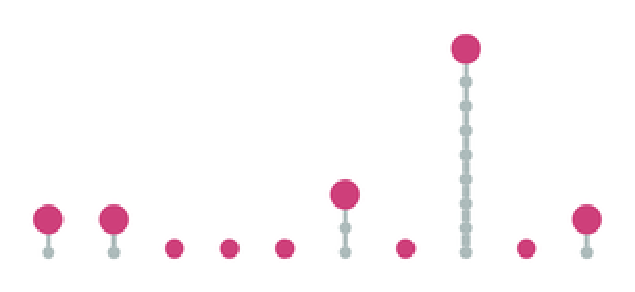
\includegraphics[scale=.25]{recAft.pdf}$
\end{lstlisting}


\subsubsection{Inducing noisy data constructors}
We generated colors for our trees using Gaussians and one motivation for this would be to model the random processes in the environment.  There is another, more subtle, reason to introduce a noise process into our programs related to representation.  Randomness in data constructors (such as \texttt{color}) can potentially allow for compact representations of patterns in the presence of noise.  To get a sense of this idea look at figure \ref{fig:noiseCons}. 
\begin{figure}[h]
\begin{center}
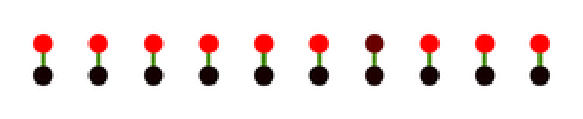
\includegraphics[scale=.60]{noisyConstructor.pdf}
\end{center}
\caption{Some trees.}
\label{fig:noiseCons}
\end{figure}
Without a noisy data constructor (i.e., if there were no Gaussian inside calls to \texttt{color}) we might create the following generative model:
\begin{lstlisting}
(if (flip)
 (node (data (color 20) (size .5)) (node (data (color 255) (size .5))))
 (node (data (color 20) (size .5)) (node (data (color 105) (size .5)))))
\end{lstlisting}
This seems like a big penalty as far as model representation size goes since the probability of drawing the darker colored object may be incredibly small.  By having a noisy constructor we can model the data more compactly as simply 
\begin{lstlisting}
(node (data (color 20) (size .5)) (node (data (color (gaussian 255 25) (size .5)))))
\end{lstlisting}

The use of the noisy color constructor in our programs was built into the \texttt{incorporate-data} function as noted earlier.  Here we give an example of how the compactness of noisy constructors might be used to ``learn'' them from data.

We make the following minor adjustments to \texttt{incorporate-data} and \texttt{noisy-number-replacement}. The first is to not have \texttt{incorporate-data} automatically add a call to \texttt{gaussian}.
\begin{lstlisting}[frame=trBLsingle]
(define (node-data->expression lst)
  `(data (color (gaussian ,(first (second lst)) 25))
	 (size ,(first (third lst)))))
\end{lstlisting}
becomes
\begin{lstlisting}[frame=trBLsingle]
(define (node-data->expression lst)
  `(data (color ,(first (second lst))) (size ,(first (third lst)))))
\end{lstlisting}
Instead of having \texttt{noisy-number-replacement} return the sample mean in a deargument move we have it return a call to the \texttt{gaussian} function and use the sample mean and variance as parameters.
\begin{lstlisting}[frame=trBL]
(define (noisy-number-replacement program abstraction variable variable-instances)
  (if (all (map number? variable-instances))
      (my-mean variable-instances)
      NO-REPLACEMENT))
\end{lstlisting}
becomes
\begin{lstlisting}[frame=trBLsingle]
(define (noisy-number-replacement program abstraction variable variable-instances)
  (if (all (map number? variable-instances))
      (let* ([instances-mean (my-mean variable-instances)]
	     [instances-deviation (sqrt (sample-variance variable-instances))])
	`(gaussian ,instances-mean ,instances-deviation))
      NO-REPLACEMENT))
\end{lstlisting}

We use the following program to generate three node structures where there is some variance in the color of the third node.
\begin{lstlisting}[mathescape=true]
(define (three-node shade)
(node (data (color 0) (size .3))
      (node (data (color 0) (size .3)) 
	    (node (data (color (gaussian shade 10)) (size .3))))))

(list (three-node 200) (three-node 200) (three-node 200) (three-node 200) (three-node 200) (three-node 200) (three-node 200) (three-node 200) (three-node 200) (three-node 200))
$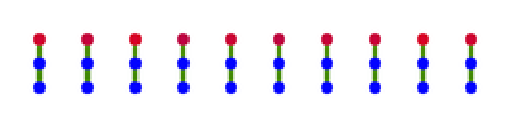
\includegraphics[scale=.6]{learnnoise-data.pdf}$
\end{lstlisting}
Data incorporation gives us a program that uniformly chooses between ten generated three node structures.
\begin{lstlisting}[mathescape=true]
(lambda ()
  (uniform-choice
   (node (data (color 0) (size 0.3))
	 (node (data (color 0) (size 0.3))
	       (node (data (color 209.0) (size 0.3)))))
   (node (data (color 0) (size 0.3))
	 (node (data (color 0) (size 0.3))
	       (node (data (color 196.0) (size 0.3)))))
                $\vdots$
   (node (data (color 0) (size 0.3))
	 (node (data (color 0) (size 0.3))
	       (node (data (color 206.0) (size 0.3)))))))
\end{lstlisting}
Bayesian program merging with the above modifications results in a compressed program that creates a function for the three node structure that adds noise to the color of the third node.  We ran the system with $\alpha=3$, beam width 1, and depth 10 for this example.
\begin{lstlisting}[mathescape=true]
(begin
    (define F2 (lambda (V2) (data (color V2) (size 0.3))))
    (define F1
      (lambda ()
        ((lambda (V1)
           (node (F2 0) (node (F2 0) (node (F2 V1)))))
          (gaussian 202.3 9.286190463980603))))
    (lambda ()
      (uniform-choice (F1) (F1) (F1) (F1) (F1) (F1) (F1)
        (F1) (F1) (F1))))
$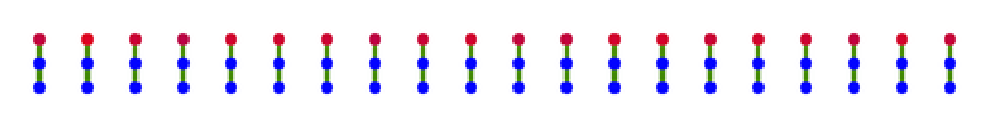
\includegraphics[scale=.6]{learnnoise-output.pdf}$
\end{lstlisting}

The discussion above hints at the benefits of using probabilistic data constructors and probabilistic programs in general with respect to representation, but understanding the full implications of such a design decision and its impact on program induction are left as future work.


\subsubsection{Deargumentation as program induction}

In some sense the problem we are trying to address with the Deargumentation is program induction itself.  We can view the values for each variable as data generated by some process we would like to identify, i.e., there is some sort of common computation between variable values that we would like to represent as a program.  In the case of the noisy-number transformation we can view the generation of values for a single variable as coming from the same process, here we restrict the program representing this process to a Gaussian.  Similarly, in the case of the recursive transformation we can view the generation of values for a single variable as coming from a the same process, but we restrict the program representing this process to be the function being deargumented.  In the case of the same variable transformation we can view the generation of values for multiple variables as coming from the same process and we implicitly use the program for one variable as the generating process for the other.  

Hence, it is natural to ask whether we could reformulate the Deargumentation transform as recursive calls to the Bayesian program merging procedure in an attempt to find programs for generating the values of the variables.  One can think of this as recursively squeezing out the randomness in the data where the abstractions created by inverse inlining create a separation between the ``structured'' parts of the data (the fixed common sub-expressions) and the random parts of the data (the variables in the expression patterns).  As an abstraction is applied one gets more data for the random parts and could conceivably attempt to learn a program to generate this data, i.e., separate out even more structure.


\newpage
\section{Examples}
\subsection{Single color flower}
We use the program below to generate ten instances of flower that have the same color.  
\begin{lstlisting}[mathescape=true]
(define (flower shade)
  (node (data (color (gaussian shade 25)) (size .3))
        (petal shade)
        (petal shade)
        (petal shade)))

(define (petal shade)
  (node (data (color (gaussian shade 25)) (size .3))))

(repeat 10 (lambda () (flower 20)))
$
\includegraphics[scale=.35]{single-color-data.pdf}$
\end{lstlisting}
An expression for these ten flowers was created using data incorporation and this expression was compressed into the program below.  The function \texttt{F1} is a function that takes no arguments and creates a flower with petals that are all the same color.  We ran the system with $\alpha=1$, beam width 1, and depth 10 for this example.
\begin{lstlisting}[mathescape=true]
(begin
  (define F2
    (lambda (V5)
      (data (color (gaussian V5 25)) (size 0.3))))
  (define F1
    (lambda ()
      ((lambda (V4)
	 ((lambda (V2)
	    ((lambda (V1)
	       ((lambda (V3)
		  (node (F2 V1) (node (F2 V2))
			(node (F2 V3)) (node (F2 V4))))
		17.2))
	     32.9))
	  2.0))
       19.7)))
  (lambda ()
    (uniform-choice (F1) (F1) (F1) (F1) (F1) (F1) (F1)
		    (F1) (F1) (F1))))

$
\includegraphics[scale=.35]{single-color-model.pdf}$
\end{lstlisting}
\subsection{Multiple color flower}
Here we use a similar program to generate ten instances of flower that have alternating colors.  
\begin{lstlisting}[mathescape=true]
(define (flower shade)
  (node (data (color (gaussian 0 25)) (size .3))
        (petal shade)
        (petal shade)
        (petal shade)))

(define (petal shade)
  (node (data (color (gaussian shade 25)) (size .3))))

(repeat 10 (lambda () (flower (if (flip) 100 220))))
$
\includegraphics[scale=.35]{paramPartsData.pdf}$
\end{lstlisting}
Bayesian program merging results in the following program.  The abstraction \texttt{F2} corresponds to \texttt{petal} and \texttt{F1} corresponds to \texttt{flower}.  We ran the system with $\alpha=1$ for this example, beam width 1, and depth 10.
\begin{lstlisting}[mathescape=true]
(begin
  (define F2
    (lambda (V5)
      (data (color (gaussian V5 25)) (size 0.3))))
  (define F1
    (lambda (V2)
      ((lambda (V1)
         ((lambda (V3)
            ((lambda (V4)
               (node (F2 V1) (node (F2 V2)) (node (F2 V3))
                     (node (F2 V4))))
             V2))
          V1))
       V2)))
  (lambda ()
    (uniform-choice (F1 91.0) (F1 85.0) (F1 254.0)
                    (F1 234.0) (F1 82.0) (F1 243.0) (F1 104.0))))
$
\includegraphics[scale=.35]{paramPartsModelData.pdf}$
\end{lstlisting}
\subsection{Recursion}
We use the following program to generate a tree made of a single line of nodes.  We ran the system with $\alpha=1$ for this example, beam width 1, and depth 10.
\begin{lstlisting}[mathescape=true]
(define (line)
  (if (flip .2)
      (node (data (color 200) (size .5)))
      (node (data (color 200) (size .5)) (line))))
$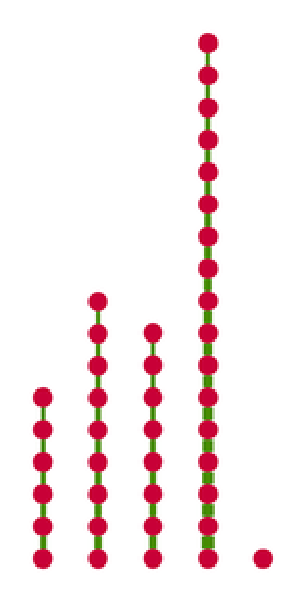
\includegraphics[scale=.35]{recursionData.pdf}$
\end{lstlisting}
Bayesian program merging finds the following recursion.
\begin{lstlisting}[mathescape=true]
(begin 
  (define F3 (lambda () (lambda () (F1))))
  (define F2
    (lambda () (data (color (gaussian 200 25)) (size 0.5))))
  (define F1
    (lambda ()
      ((lambda (V1) (node (F2) V1))
       (if (flip 8/9) (F1) (node (F2))))))
  (lambda ()
    (uniform-choice
     (list (F3) (F3) (F3) (F3) (lambda () (node (F2))))))))
$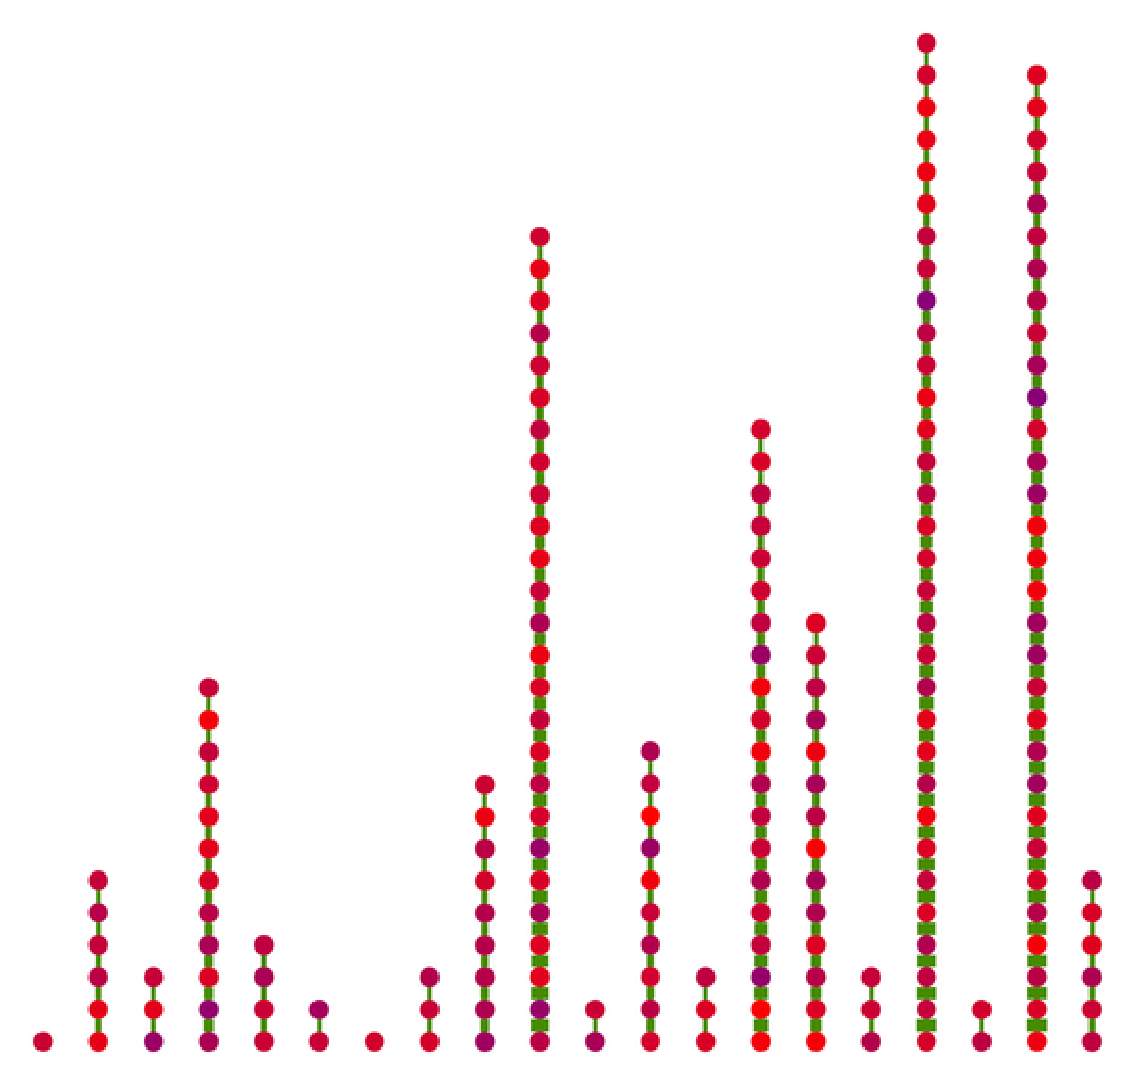
\includegraphics[scale=.25]{recursionModel.pdf}$
\end{lstlisting}
The recursions have to be of a certain length before the tradeoff between prior and likelihood favors the recursive programs, which are usually smaller.  We can adjust where this tradeoff happens using the size constant, $\alpha$, in the prior. 
\subsection{Vine}
Here we use Bayesian program merging to model a vine with flowers from a single instance.  This example demonstrates multiple types of program transformations used on the same data.  We ran the system with $\alpha=1$ for this example, beam width 1, and depth 10.
\begin{lstlisting}[mathescape=true]
(define (vine)
  (if (flip .1)
      (node (data (color 100) (size .1)))
      (node (data (color 100) (size .1)) (vine) (flower))))

(define (flower)
  (node (data (color (gaussian 20 25)) (size .3))
        (petal 20)
        (petal 20)))

(define (petal shade)
  (node (data (color (gaussian shade 25)) (size .3))))
$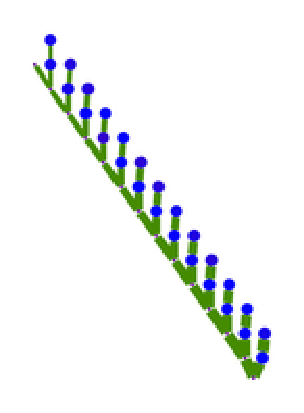
\includegraphics[scale=.35]{vineData.pdf}$
\end{lstlisting}
Here we see \texttt{F1} corresponds roughly to \texttt{vine} and is passed a single color for the flower parts and the size has been fixed within \texttt{F1}, \texttt{F2} corresponds to the data part of the flower.
\begin{lstlisting}[mathescape=true]
(begin
  (define F3 (lambda () (F2 100 0.1)))
  (define F2
    (lambda (V4 V5)
      (data (color (gaussian V4 25)) (size V5))))
  (define F1
    (lambda (V2)
      ((lambda (V3)
         ((lambda (V1)
            (node (F3) V1
                  (node (F2 V2 0.3) (node (F2 V3 0.3)))))
          (if (flip 12/13) (F1 1.0) (node (F3)))))
       7.0)))
  (lambda ()
    (uniform-choice (F1 -14.0))))
$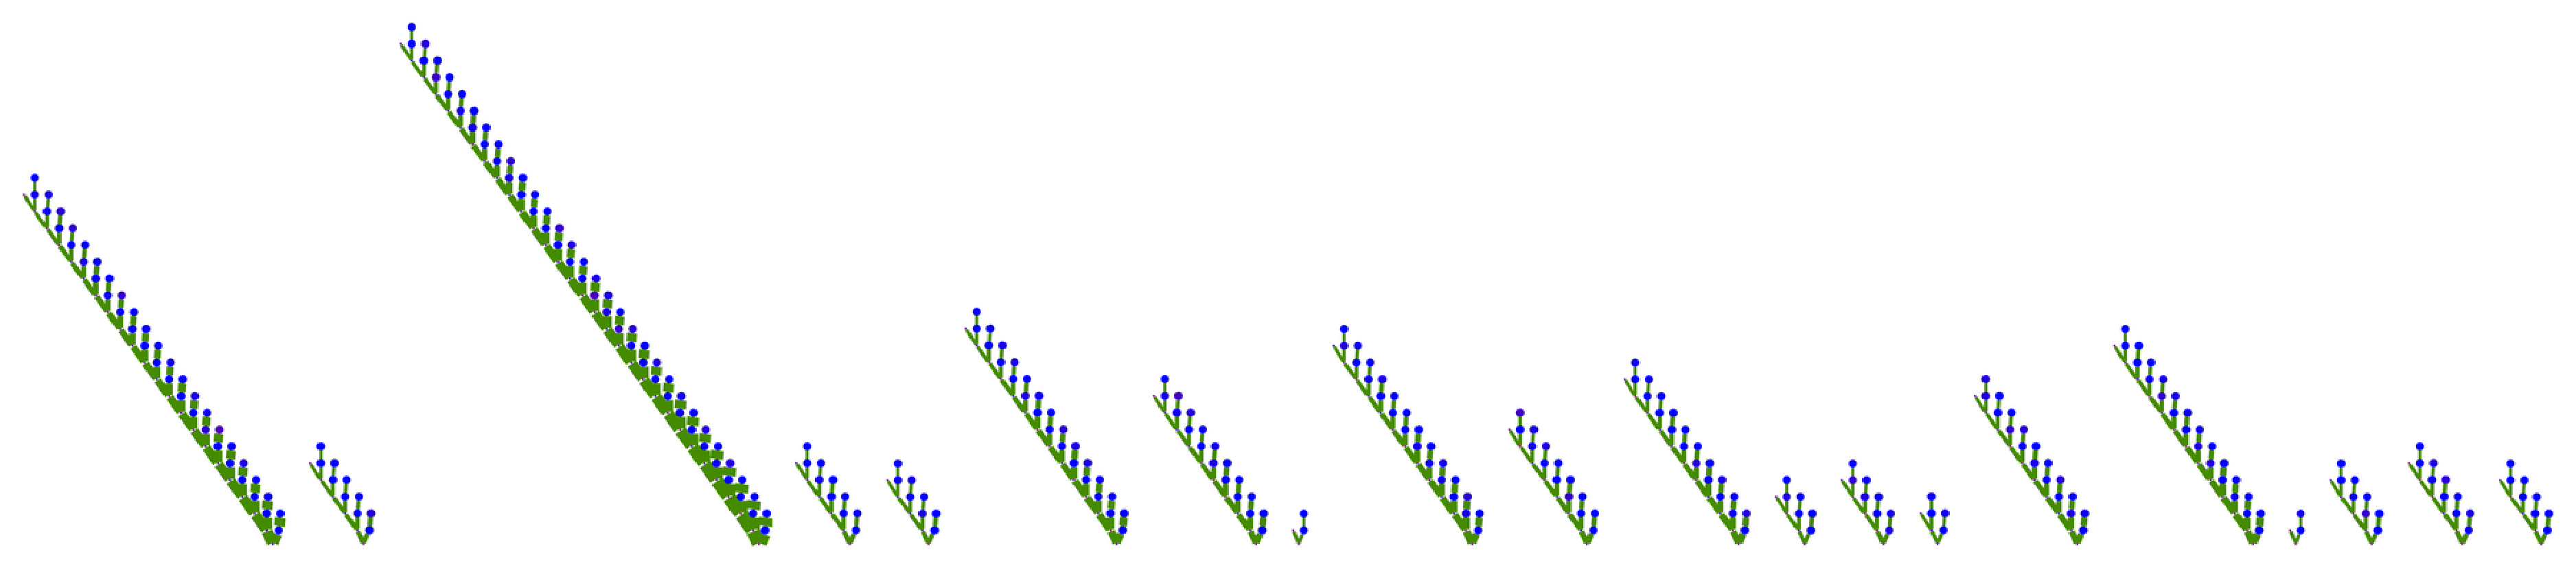
\includegraphics[scale=.25]{vineModel.pdf}$
\end{lstlisting}
\subsection{Tree}
This example demonstrates learning both a parameterized function and a recursion and applying these functions in multiple places within a program.  The following functions were used to generate some flower patterns and a tree that consists of two branches each of which ends in a different color flower.  We ran the system with $\alpha=3$, beam width 1, and depth 10 for this example.  With $\alpha=1$ we do not get the right tradeoff between prior and likelihood to make introducing recursion worhtwhile although We expect the system could learn a similar program with $\alpha=1$ given training examples with more branch instances, since the amount of program compression would increase.
\begin{lstlisting}[mathescape=true]
(define tree
  (lambda ()
    (uniform-choice
     (node (body) (branch) (branch)))))

(define (body) 
  (data (color (gaussian 50 25)) (size 1)))

(define (branch)
  (if (flip .1)
      (uniform-choice (flower 20) (flower 220))
      (node (branch-info) (branch))))

(define (branch-info)
  (data (color (gaussian 100 25)) (size .1)))

(define (flower shade)
  (node (data (color (gaussian shade 25)) (size .3))
        (petal shade)
        (petal shade)))

(define (petal shade)
  (node (data (color (gaussian shade 25)) (size .3))))
$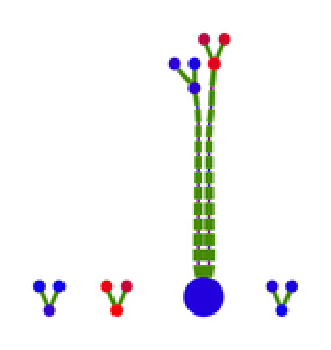
\includegraphics[scale=.25]{treeData.pdf}$
\end{lstlisting}
Bayesian model merging produces a program with a similar structure to the original generating program.  \texttt{F3} plays a similar role to the \texttt{flower} function by taking a single color as argument and creating three nodes of size .3 with the passed in color.  \texttt{F2} is a function that creates a branch that ends in a flower with either blue petals or red petals.
\begin{lstlisting}[mathescape=true]
(begin
   (define F4 (lambda (V9 V10) (node (F1 V9 0.1) V10)))
   (define F3
     (lambda (V7)
       ((lambda (V6)
          ((lambda (V8)
             (node (F1 V6 0.3) (node (F1 V7 0.3))
                   (node (F1 V8 0.3))))
           V7))
        V7)))
   (define F2
     (lambda (V3 V4)
       ((lambda (V5) (F4 V3 (F4 V4 V5)))
        (if (flip 9/11)
            (F2 121.0 135.0)
            (uniform-choice (F4 39.0 (F3 47.0)) (F3 187.0))))))
   (define F1
     (lambda (V1 V2)
       (data (color (gaussian V1 25)) (size V2))))
   (lambda ()
     (uniform-choice (F3 2e1) (F3 235.0)
                     (node (F1 34.0 1) (F2 108.0 99.0) (F2 134.0 85.0))
                     (F3 36.0))))
$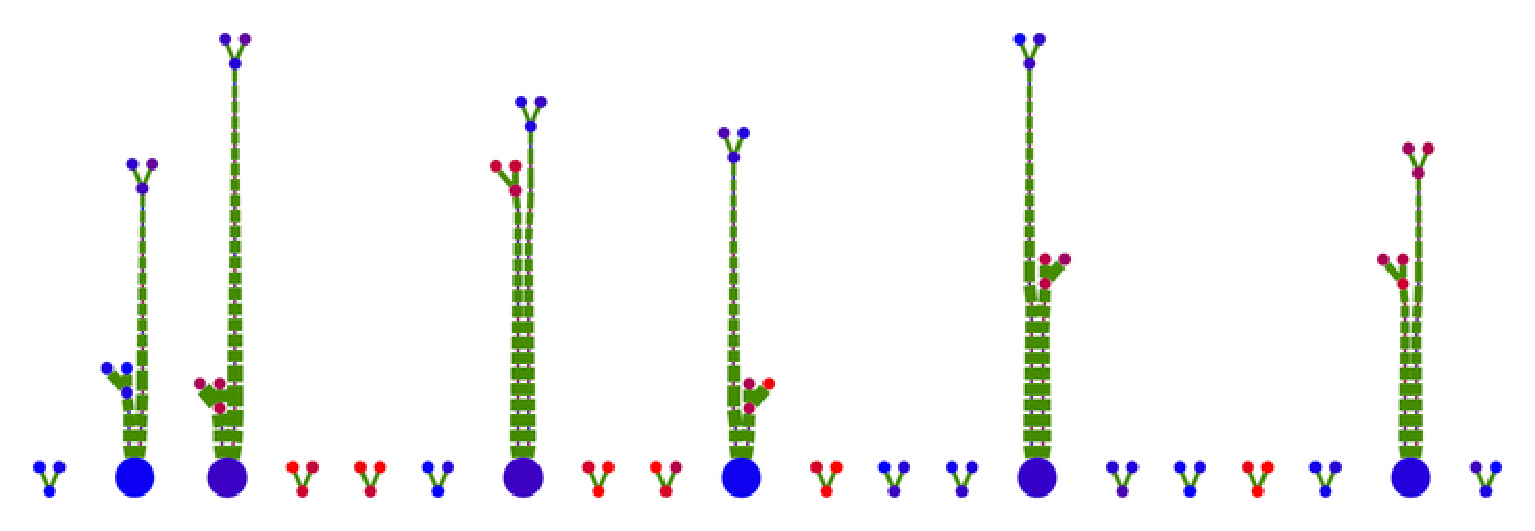
\includegraphics[scale=.25]{treeModel.pdf}$
\end{lstlisting}


\newpage
\section{Conclusion}
We presented Bayesian program merging, an approach to inducing generative models from data. The main idea of this approach is to directly translate the data into a program and to then compress this program by identifying repeated computations. We perform this compression of repeated computation using program transformations. We determine the sequence of transformations by using the posterior probability of the program as a search heuristic.

Future improvements of the system described in this paper include more sophisticated search strategies, more efficient ways of computing the likelihood, and the development of a more robust method for identifying recursive patterns.  Another direction is adaptation of this style of probabilistic program induction to the online setting.  

More generally, we can ask whether the idea of regularity in data as repeated computation in the generative process can be used to identify other useful program transformations or, whether it can be applied in a more systematic fashion than motivating a collection of disparate search moves.  

A different and important question is what happens when the data incorporation step is less immediate and training data is not directly computed in terms of some algebraic data type and whether one can impose some semblance of structure on unstructured data in order to use these methods for learning.  

There are many other barriers to overcome before probabilistic program induction can compete with state-of-the-art machine learning algorithms on real world problems, but the increased potential for capturing rich patterns and less dependence on human engineering make research in the subject a worthy pursuit.
\bibliographystyle{plain}
\bibliography{myBib}
\end{document}
